\panel{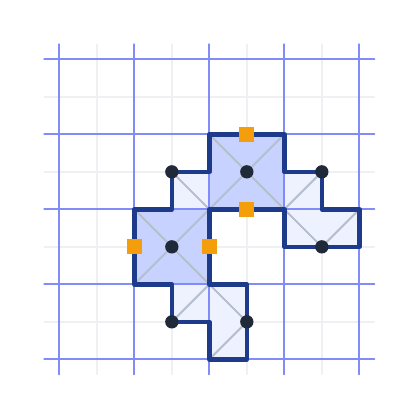
\begin{tikzpicture}[x=1bp, y=1bp]\path[use as bounding box] (0,0) rectangle (130.80,130.80);\clip (0,0) rectangle (130.80,130.80);
\path[draw={rgb,255:red,238;green,240;blue,243}, line width=0.52bp, line cap=round, line join=round] (11.40,6.00) -- (11.40,124.80);
\path[draw={rgb,255:red,238;green,240;blue,243}, line width=0.52bp, line cap=round, line join=round] (24.90,6.00) -- (24.90,124.80);
\path[draw={rgb,255:red,238;green,240;blue,243}, line width=0.52bp, line cap=round, line join=round] (38.40,6.00) -- (38.40,124.80);
\path[draw={rgb,255:red,238;green,240;blue,243}, line width=0.52bp, line cap=round, line join=round] (51.90,6.00) -- (51.90,124.80);
\path[draw={rgb,255:red,238;green,240;blue,243}, line width=0.52bp, line cap=round, line join=round] (65.40,6.00) -- (65.40,124.80);
\path[draw={rgb,255:red,238;green,240;blue,243}, line width=0.52bp, line cap=round, line join=round] (78.90,6.00) -- (78.90,124.80);
\path[draw={rgb,255:red,238;green,240;blue,243}, line width=0.52bp, line cap=round, line join=round] (92.40,6.00) -- (92.40,124.80);
\path[draw={rgb,255:red,238;green,240;blue,243}, line width=0.52bp, line cap=round, line join=round] (105.90,6.00) -- (105.90,124.80);
\path[draw={rgb,255:red,238;green,240;blue,243}, line width=0.52bp, line cap=round, line join=round] (119.40,6.00) -- (119.40,124.80);
\path[draw={rgb,255:red,238;green,240;blue,243}, line width=0.52bp, line cap=round, line join=round] (6.00,11.40) -- (124.80,11.40);
\path[draw={rgb,255:red,238;green,240;blue,243}, line width=0.52bp, line cap=round, line join=round] (6.00,24.90) -- (124.80,24.90);
\path[draw={rgb,255:red,238;green,240;blue,243}, line width=0.52bp, line cap=round, line join=round] (6.00,38.40) -- (124.80,38.40);
\path[draw={rgb,255:red,238;green,240;blue,243}, line width=0.52bp, line cap=round, line join=round] (6.00,51.90) -- (124.80,51.90);
\path[draw={rgb,255:red,238;green,240;blue,243}, line width=0.52bp, line cap=round, line join=round] (6.00,65.40) -- (124.80,65.40);
\path[draw={rgb,255:red,238;green,240;blue,243}, line width=0.52bp, line cap=round, line join=round] (6.00,78.90) -- (124.80,78.90);
\path[draw={rgb,255:red,238;green,240;blue,243}, line width=0.52bp, line cap=round, line join=round] (6.00,92.40) -- (124.80,92.40);
\path[draw={rgb,255:red,238;green,240;blue,243}, line width=0.52bp, line cap=round, line join=round] (6.00,105.90) -- (124.80,105.90);
\path[draw={rgb,255:red,238;green,240;blue,243}, line width=0.52bp, line cap=round, line join=round] (6.00,119.40) -- (124.80,119.40);
\path[fill={rgb,255:red,238;green,242;blue,255}] (38.40,38.40) rectangle (51.90,51.90);
\path[fill={rgb,255:red,238;green,242;blue,255}] (51.90,38.40) rectangle (65.40,51.90);
\path[fill={rgb,255:red,238;green,242;blue,255}] (51.90,24.90) rectangle (65.40,38.40);
\path[fill={rgb,255:red,238;green,242;blue,255}] (65.40,24.90) rectangle (78.90,38.40);
\path[fill={rgb,255:red,238;green,242;blue,255}] (65.40,11.40) rectangle (78.90,24.90);
\path[fill={rgb,255:red,238;green,242;blue,255}] (38.40,51.90) rectangle (51.90,65.40);
\path[fill={rgb,255:red,238;green,242;blue,255}] (51.90,51.90) rectangle (65.40,65.40);
\path[fill={rgb,255:red,238;green,242;blue,255}] (51.90,65.40) rectangle (65.40,78.90);
\path[fill={rgb,255:red,238;green,242;blue,255}] (65.40,65.40) rectangle (78.90,78.90);
\path[fill={rgb,255:red,238;green,242;blue,255}] (65.40,78.90) rectangle (78.90,92.40);
\path[fill={rgb,255:red,238;green,242;blue,255}] (105.90,51.90) rectangle (119.40,65.40);
\path[fill={rgb,255:red,238;green,242;blue,255}] (92.40,51.90) rectangle (105.90,65.40);
\path[fill={rgb,255:red,238;green,242;blue,255}] (92.40,65.40) rectangle (105.90,78.90);
\path[fill={rgb,255:red,238;green,242;blue,255}] (78.90,65.40) rectangle (92.40,78.90);
\path[fill={rgb,255:red,238;green,242;blue,255}] (78.90,78.90) rectangle (92.40,92.40);
\path[fill={rgb,255:red,199;green,210;blue,254}] (65.40,65.40) rectangle (92.40,92.40);
\path[fill={rgb,255:red,199;green,210;blue,254}] (38.40,38.40) rectangle (65.40,65.40);
\path[draw={rgb,255:red,182;green,191;blue,208}, line width=0.60bp, line cap=round, line join=round] (51.90,51.90) -- (38.40,38.40);
\path[draw={rgb,255:red,182;green,191;blue,208}, line width=0.60bp, line cap=round, line join=round] (51.90,51.90) -- (38.40,38.40);
\path[draw={rgb,255:red,182;green,191;blue,208}, line width=0.60bp, line cap=round, line join=round] (51.90,51.90) -- (65.40,38.40);
\path[draw={rgb,255:red,182;green,191;blue,208}, line width=0.60bp, line cap=round, line join=round] (51.90,51.90) -- (65.40,38.40);
\path[draw={rgb,255:red,182;green,191;blue,208}, line width=0.60bp, line cap=round, line join=round] (51.90,24.90) -- (65.40,38.40);
\path[draw={rgb,255:red,182;green,191;blue,208}, line width=0.60bp, line cap=round, line join=round] (51.90,24.90) -- (65.40,38.40);
\path[draw={rgb,255:red,182;green,191;blue,208}, line width=0.60bp, line cap=round, line join=round] (78.90,24.90) -- (65.40,38.40);
\path[draw={rgb,255:red,182;green,191;blue,208}, line width=0.60bp, line cap=round, line join=round] (78.90,24.90) -- (65.40,38.40);
\path[draw={rgb,255:red,182;green,191;blue,208}, line width=0.60bp, line cap=round, line join=round] (78.90,24.90) -- (65.40,11.40);
\path[draw={rgb,255:red,182;green,191;blue,208}, line width=0.60bp, line cap=round, line join=round] (78.90,24.90) -- (65.40,11.40);
\path[draw={rgb,255:red,182;green,191;blue,208}, line width=0.60bp, line cap=round, line join=round] (51.90,51.90) -- (38.40,65.40);
\path[draw={rgb,255:red,182;green,191;blue,208}, line width=0.60bp, line cap=round, line join=round] (51.90,51.90) -- (38.40,65.40);
\path[draw={rgb,255:red,182;green,191;blue,208}, line width=0.60bp, line cap=round, line join=round] (51.90,51.90) -- (65.40,65.40);
\path[draw={rgb,255:red,182;green,191;blue,208}, line width=0.60bp, line cap=round, line join=round] (51.90,51.90) -- (65.40,65.40);
\path[draw={rgb,255:red,182;green,191;blue,208}, line width=0.60bp, line cap=round, line join=round] (51.90,78.90) -- (65.40,65.40);
\path[draw={rgb,255:red,182;green,191;blue,208}, line width=0.60bp, line cap=round, line join=round] (51.90,78.90) -- (65.40,65.40);
\path[draw={rgb,255:red,182;green,191;blue,208}, line width=0.60bp, line cap=round, line join=round] (78.90,78.90) -- (65.40,65.40);
\path[draw={rgb,255:red,182;green,191;blue,208}, line width=0.60bp, line cap=round, line join=round] (78.90,78.90) -- (65.40,65.40);
\path[draw={rgb,255:red,182;green,191;blue,208}, line width=0.60bp, line cap=round, line join=round] (78.90,78.90) -- (65.40,92.40);
\path[draw={rgb,255:red,182;green,191;blue,208}, line width=0.60bp, line cap=round, line join=round] (78.90,78.90) -- (65.40,92.40);
\path[draw={rgb,255:red,182;green,191;blue,208}, line width=0.60bp, line cap=round, line join=round] (105.90,51.90) -- (119.40,65.40);
\path[draw={rgb,255:red,182;green,191;blue,208}, line width=0.60bp, line cap=round, line join=round] (105.90,51.90) -- (119.40,65.40);
\path[draw={rgb,255:red,182;green,191;blue,208}, line width=0.60bp, line cap=round, line join=round] (105.90,51.90) -- (92.40,65.40);
\path[draw={rgb,255:red,182;green,191;blue,208}, line width=0.60bp, line cap=round, line join=round] (105.90,51.90) -- (92.40,65.40);
\path[draw={rgb,255:red,182;green,191;blue,208}, line width=0.60bp, line cap=round, line join=round] (105.90,78.90) -- (92.40,65.40);
\path[draw={rgb,255:red,182;green,191;blue,208}, line width=0.60bp, line cap=round, line join=round] (105.90,78.90) -- (92.40,65.40);
\path[draw={rgb,255:red,182;green,191;blue,208}, line width=0.60bp, line cap=round, line join=round] (78.90,78.90) -- (92.40,65.40);
\path[draw={rgb,255:red,182;green,191;blue,208}, line width=0.60bp, line cap=round, line join=round] (78.90,78.90) -- (92.40,65.40);
\path[draw={rgb,255:red,182;green,191;blue,208}, line width=0.60bp, line cap=round, line join=round] (78.90,78.90) -- (92.40,92.40);
\path[draw={rgb,255:red,182;green,191;blue,208}, line width=0.60bp, line cap=round, line join=round] (78.90,78.90) -- (92.40,92.40);
\path[draw={rgb,255:red,129;green,140;blue,248}, line width=0.83bp, line cap=round, line join=round] (11.40,6.00) -- (11.40,124.80);
\path[draw={rgb,255:red,129;green,140;blue,248}, line width=0.83bp, line cap=round, line join=round] (6.00,11.40) -- (124.80,11.40);
\path[draw={rgb,255:red,129;green,140;blue,248}, line width=0.83bp, line cap=round, line join=round] (38.40,6.00) -- (38.40,124.80);
\path[draw={rgb,255:red,129;green,140;blue,248}, line width=0.83bp, line cap=round, line join=round] (6.00,38.40) -- (124.80,38.40);
\path[draw={rgb,255:red,129;green,140;blue,248}, line width=0.83bp, line cap=round, line join=round] (65.40,6.00) -- (65.40,124.80);
\path[draw={rgb,255:red,129;green,140;blue,248}, line width=0.83bp, line cap=round, line join=round] (6.00,65.40) -- (124.80,65.40);
\path[draw={rgb,255:red,129;green,140;blue,248}, line width=0.83bp, line cap=round, line join=round] (92.40,6.00) -- (92.40,124.80);
\path[draw={rgb,255:red,129;green,140;blue,248}, line width=0.83bp, line cap=round, line join=round] (6.00,92.40) -- (124.80,92.40);
\path[draw={rgb,255:red,129;green,140;blue,248}, line width=0.83bp, line cap=round, line join=round] (119.40,6.00) -- (119.40,124.80);
\path[draw={rgb,255:red,129;green,140;blue,248}, line width=0.83bp, line cap=round, line join=round] (6.00,119.40) -- (124.80,119.40);
\path[draw={rgb,255:red,30;green,58;blue,138}, line width=1.65bp, line join=round] (38.40,38.40) -- (38.40,65.40) -- (51.90,65.40) -- (51.90,78.90) -- (65.40,78.90) -- (65.40,92.40) -- (92.40,92.40) -- (92.40,78.90) -- (105.90,78.90) -- (105.90,65.40) -- (119.40,65.40) -- (119.40,51.90) -- (92.40,51.90) -- (92.40,65.40) -- (65.40,65.40) -- (65.40,38.40) -- (78.90,38.40) -- (78.90,11.40) -- (65.40,11.40) -- (65.40,24.90) -- (51.90,24.90) -- (51.90,38.40) -- cycle;
\path[fill={rgb,255:red,31;green,41;blue,55}] (51.90,78.90) circle[radius=2.40bp];
\path[fill={rgb,255:red,31;green,41;blue,55}] (105.90,78.90) circle[radius=2.40bp];
\path[fill={rgb,255:red,31;green,41;blue,55}] (51.90,51.90) circle[radius=2.40bp];
\path[fill={rgb,255:red,31;green,41;blue,55}] (78.90,78.90) circle[radius=2.40bp];
\path[fill={rgb,255:red,31;green,41;blue,55}] (105.90,51.90) circle[radius=2.40bp];
\path[fill={rgb,255:red,31;green,41;blue,55}] (78.90,24.90) circle[radius=2.40bp];
\path[fill={rgb,255:red,31;green,41;blue,55}] (51.90,24.90) circle[radius=2.40bp];
\path[fill={rgb,255:red,245;green,158;blue,11}] (35.70,49.20) rectangle (41.10,54.60);
\path[fill={rgb,255:red,245;green,158;blue,11}] (62.70,49.20) rectangle (68.10,54.60);
\path[fill={rgb,255:red,245;green,158;blue,11}] (76.20,62.70) rectangle (81.60,68.10);
\path[fill={rgb,255:red,245;green,158;blue,11}] (76.20,89.70) rectangle (81.60,95.10);
\end{tikzpicture}}{(a) Your room, cut into stars}\hspace{36.0bp}\panel{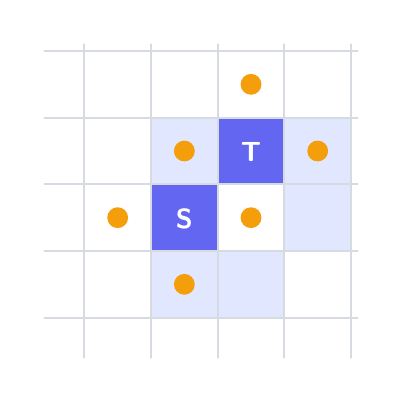
\begin{tikzpicture}[x=1bp, y=1bp]\path[use as bounding box] (0,0) rectangle (124.80,124.80);\clip (0,0) rectangle (124.80,124.80);
\path[fill={rgb,255:red,224;green,231;blue,255}] (44.40,68.40) rectangle (68.40,92.40);
\path[fill={rgb,255:red,224;green,231;blue,255}] (92.40,68.40) rectangle (116.40,92.40);
\path[fill={rgb,255:red,224;green,231;blue,255}] (92.40,44.40) rectangle (116.40,68.40);
\path[fill={rgb,255:red,224;green,231;blue,255}] (68.40,20.40) rectangle (92.40,44.40);
\path[fill={rgb,255:red,224;green,231;blue,255}] (44.40,20.40) rectangle (68.40,44.40);
\path[fill={rgb,255:red,99;green,102;blue,241}] (68.40,68.40) rectangle (92.40,92.40);
\path[fill={rgb,255:red,99;green,102;blue,241}] (44.40,44.40) rectangle (68.40,68.40);
\path[draw={rgb,255:red,214;green,218;blue,225}, line width=0.68bp, line cap=round, line join=round] (20.40,6.00) -- (20.40,118.80);
\path[draw={rgb,255:red,214;green,218;blue,225}, line width=0.68bp, line cap=round, line join=round] (44.40,6.00) -- (44.40,118.80);
\path[draw={rgb,255:red,214;green,218;blue,225}, line width=0.68bp, line cap=round, line join=round] (68.40,6.00) -- (68.40,118.80);
\path[draw={rgb,255:red,214;green,218;blue,225}, line width=0.68bp, line cap=round, line join=round] (92.40,6.00) -- (92.40,118.80);
\path[draw={rgb,255:red,214;green,218;blue,225}, line width=0.68bp, line cap=round, line join=round] (116.40,6.00) -- (116.40,118.80);
\path[draw={rgb,255:red,214;green,218;blue,225}, line width=0.68bp, line cap=round, line join=round] (6.00,20.40) -- (118.80,20.40);
\path[draw={rgb,255:red,214;green,218;blue,225}, line width=0.68bp, line cap=round, line join=round] (6.00,44.40) -- (118.80,44.40);
\path[draw={rgb,255:red,214;green,218;blue,225}, line width=0.68bp, line cap=round, line join=round] (6.00,68.40) -- (118.80,68.40);
\path[draw={rgb,255:red,214;green,218;blue,225}, line width=0.68bp, line cap=round, line join=round] (6.00,92.40) -- (118.80,92.40);
\path[draw={rgb,255:red,214;green,218;blue,225}, line width=0.68bp, line cap=round, line join=round] (6.00,116.40) -- (118.80,116.40);
\path[fill={rgb,255:red,245;green,158;blue,11}] (56.40,80.40) circle[radius=3.75bp];
\path[fill={rgb,255:red,245;green,158;blue,11}] (80.40,104.40) circle[radius=3.75bp];
\path[fill={rgb,255:red,245;green,158;blue,11}] (104.40,80.40) circle[radius=3.75bp];
\path[fill={rgb,255:red,245;green,158;blue,11}] (32.40,56.40) circle[radius=3.75bp];
\path[fill={rgb,255:red,245;green,158;blue,11}] (80.40,56.40) circle[radius=3.75bp];
\path[fill={rgb,255:red,245;green,158;blue,11}] (56.40,32.40) circle[radius=3.75bp];
\node[anchor=base, text=white, font=\fontsize{9.8}{11.7}\selectfont\sffamily\bfseries, inner sep=0pt] at (56.40,52.65) {S};
\node[anchor=base, text=white, font=\fontsize{9.8}{11.7}\selectfont\sffamily\bfseries, inner sep=0pt] at (80.40,76.65) {T};
\end{tikzpicture}}{(b) Each star shrunk to one cell}
